%# -*- coding:utf-8 -*-
\section{实验与结果}
\label{sec7-3}

\subsection{Original Data and Experimental Setup}

Considering our aim and the requirements on the computation resources, the volume containing the whole heart was extracted from the original one that include the whole body trunk of an anonymous patient. %
The dataset, in resolution of $0.4\text{mm} \times 0.4\text{mm} \times 0.6\text{mm}$, was acquired on a 128-slice CT modality (Siemens SOMATOM Definition Flash).
\begin{figure}[t]
\centering
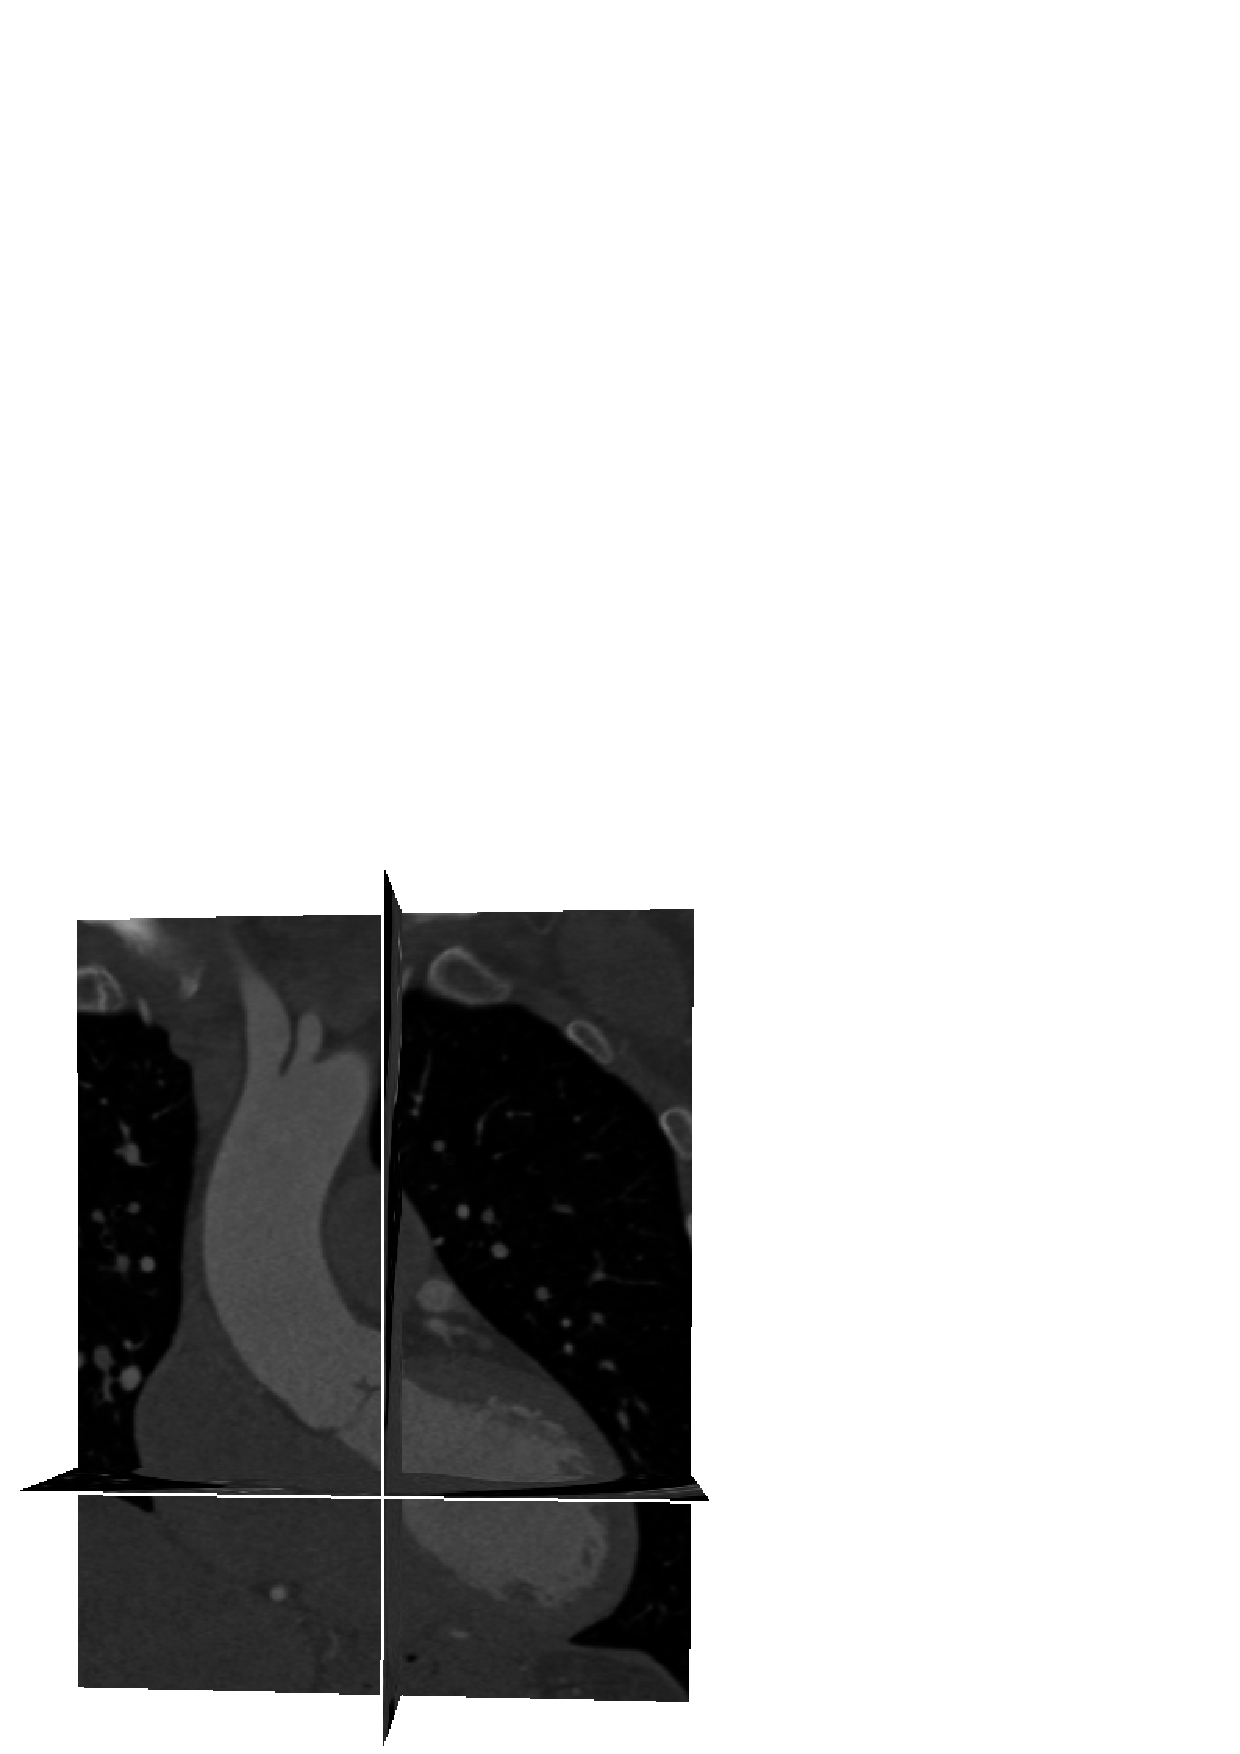
\includegraphics[height=2.0in]{Figures/chap07/original.pdf}
\caption{The anterior view of the original volume contains the whole heart extracted from the raw CT information.}
\label{fig:Original}
\end{figure}
\begin{figure}[t]
\centering
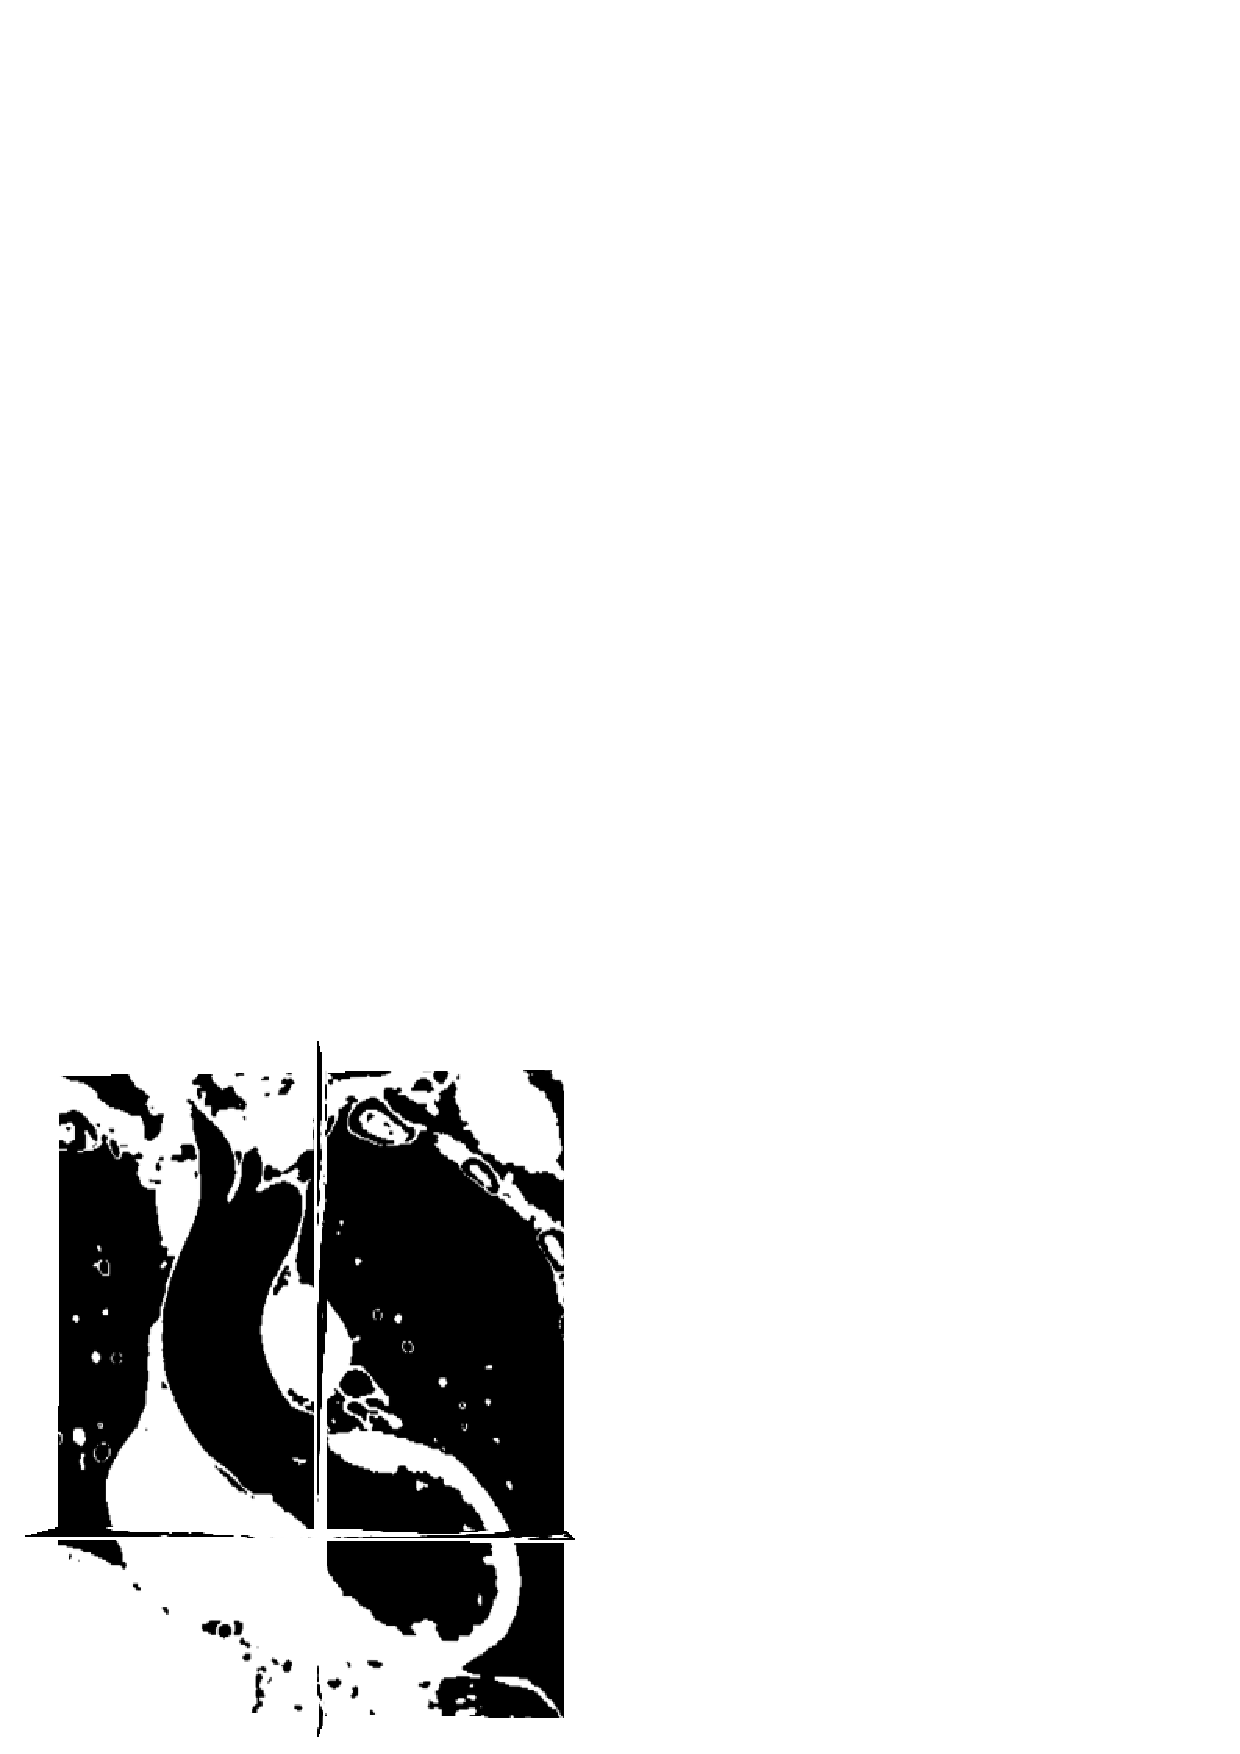
\includegraphics[height=2.0in]{Figures/chap07/binary_threshold.pdf}
\caption{Volume after binary threshold processing. Note that the pericardium, and most of the blood vessels are excluded.}%
\label{fig:BinaryThreshold}
\end{figure}

Numbers of experimental trials were carried out on the image dataset, applying distinct sets of parameters for the evaluation of the approach.
%In our case, the CTA series in DICOM format had been converted to the form of XML first.
%Then the converted data was fed into the feature image production branch and input level sets generation branch.
%The resulting data from the two branches were sent to geodesic active contours module in order to generate the final results.
%Finally, the marching cubes method is used to visualize the segmented data.
The experiments were executed on a desktop machine armed with Intel's 2.83GHz Core 2 Quad CPU and 4GB RAM.

\subsection{Preprocessing}

As mentioned in Sec. \ref{sec:overview}, series of preprocessing were conducted before the evolution of the ``snakes":
(i) the image smoothing preserving the edges;
(ii) the exclusion of the uninterested image details;
(iii) the calculation of the image gradient magnitude;
(iv) the generation of the initial contours.

As the first step, an algorithm based on MCDE given by (\ref{eqn:MCDE}) was utilized to smooth the input images.
By applying this numerical method, the edges in the images were well protected from the smoothing effect.

Then the binary thresholding was applied to archived the goal -- excluding most uninteresting contents, i.e., only the contents of interest were left after this step.
To achieve this goal, the properly chosen threshold pairs were decided based on the analysis of the histogram of the smoothing images.
Figure \ref{fig:BinaryThreshold} depicted the results of the binary thresholding step.

After thresholding the images, the rest two steps (the calculation of the edge potential and the initial contours) were performed simultaneously.

In calculating the edge potential of the images, the work was divided into two consecutive steps:
Firstly, the gradient magnitude of the images were calculated by solving (\ref{eqn:Gaussian}).
Secondly, the results of the previous step were converted into the appearance that the edges are dark while the rest of the images are bright.
In converting the gradient images, the selection of the parameters $m$ and $n$ in (\ref{eqn:Sigmoid}) were essential.
Their values depended the two extreme intensities of the pixels in the gradient images.
In the experiments, the guideline of the selection was: $m < 0$, and $n > 0$, where $n > |m|$.
The resultant images demonstrated the edges of the objects in zero intensity while the inside/outside areas in the maximum intensity (i.e., $255$).
%\begin{figure*}[t]
%\centering
%\subfloat[]{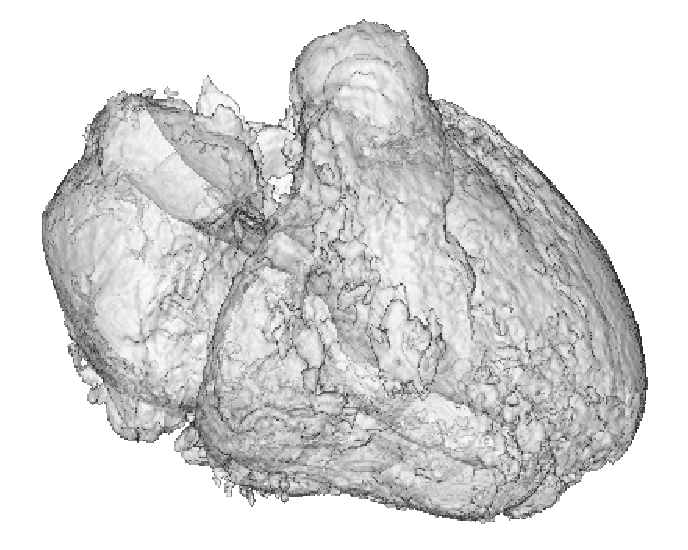
\includegraphics[height=2.5in]{../Figures/heart.eps}
%\label{fig:Heart}}
%\hfil
%\subfloat[]{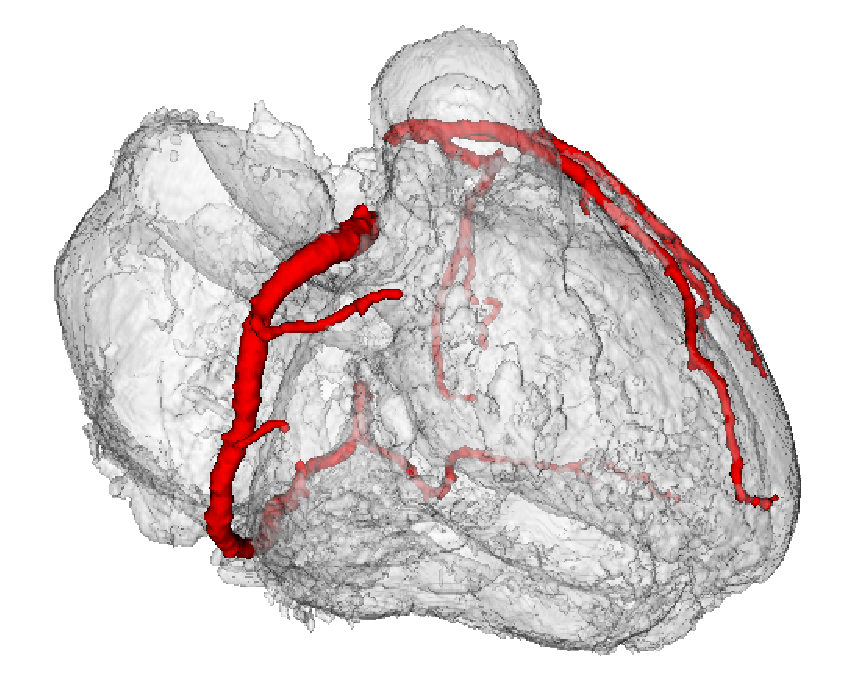
\includegraphics[height=2.5in]{../Figures/heart_with_ca.eps}
%\label{fig:Overlay}}
%\caption{The resultant models of this paper. (a) the three-dimensional model of the heart; (b) the overlayed three-dimensional models of the heart and the coronary arteries acquired in the previous work \cite{Yang2013ROBIO} are rendered in the same scene.}%
%\label{fig:HeartModel}
%\end{figure*}

Meanwhile, the evolution, driven by the fast marching algorithm \cite{Sethian1999}, started with the aim of generating the initial contours for the geodesic ``snakes" computation.
The results provided the geodesic computation the \emph{time-crossing} map so that the ``snakes" can evolve according to the computed time-of-arrival.
In this step, the only human intervention was the selection of the input seeding points, from which the computation would begin.
The location of the seeds should be located interior of the targets, and the sign of the speed function $F$ in (\ref{eqn:Eikonal}) should be positive to ensure outwards propagation of the contours. %

\subsection{Level Set Computation of Geodesic ``Snakes"}

The evolution of the geodesic ``snakes" started from the seeding points fed in previous step for the generation of the initial contours.
The ``snakes" utilized the resultant initial contours as the map in which all the pixels were marked with the time when the fronts ever crossed them.
On the other hand, that edge potential maps depicted the general geometric feature of the images, in which the magnitudes of the gradients were calculated and represented to show the ``valleys" and the ``plains" in the images. %

In order to speed up the calculation, sufficient ``attraction" in (\ref{eqn:GeodesicDriver}) was required.
Besides, the disturbance of the false edges during the evolution can be avoided due to larger attraction.
In this work, the original contours were located inside of the targets, meaning that they evolved ``outwards" towards the edges.
During the computation, the speed of the propagation was fast on the ``plains" (i.e., the inner areas of the targets), and was pretty slow when falling into the ``valleys" (i.e., the edges of the targets). %
To terminate the computation in time, the numbers of the iterations was set to $500$ in the experiments.
\begin{figure}[t]
\centering
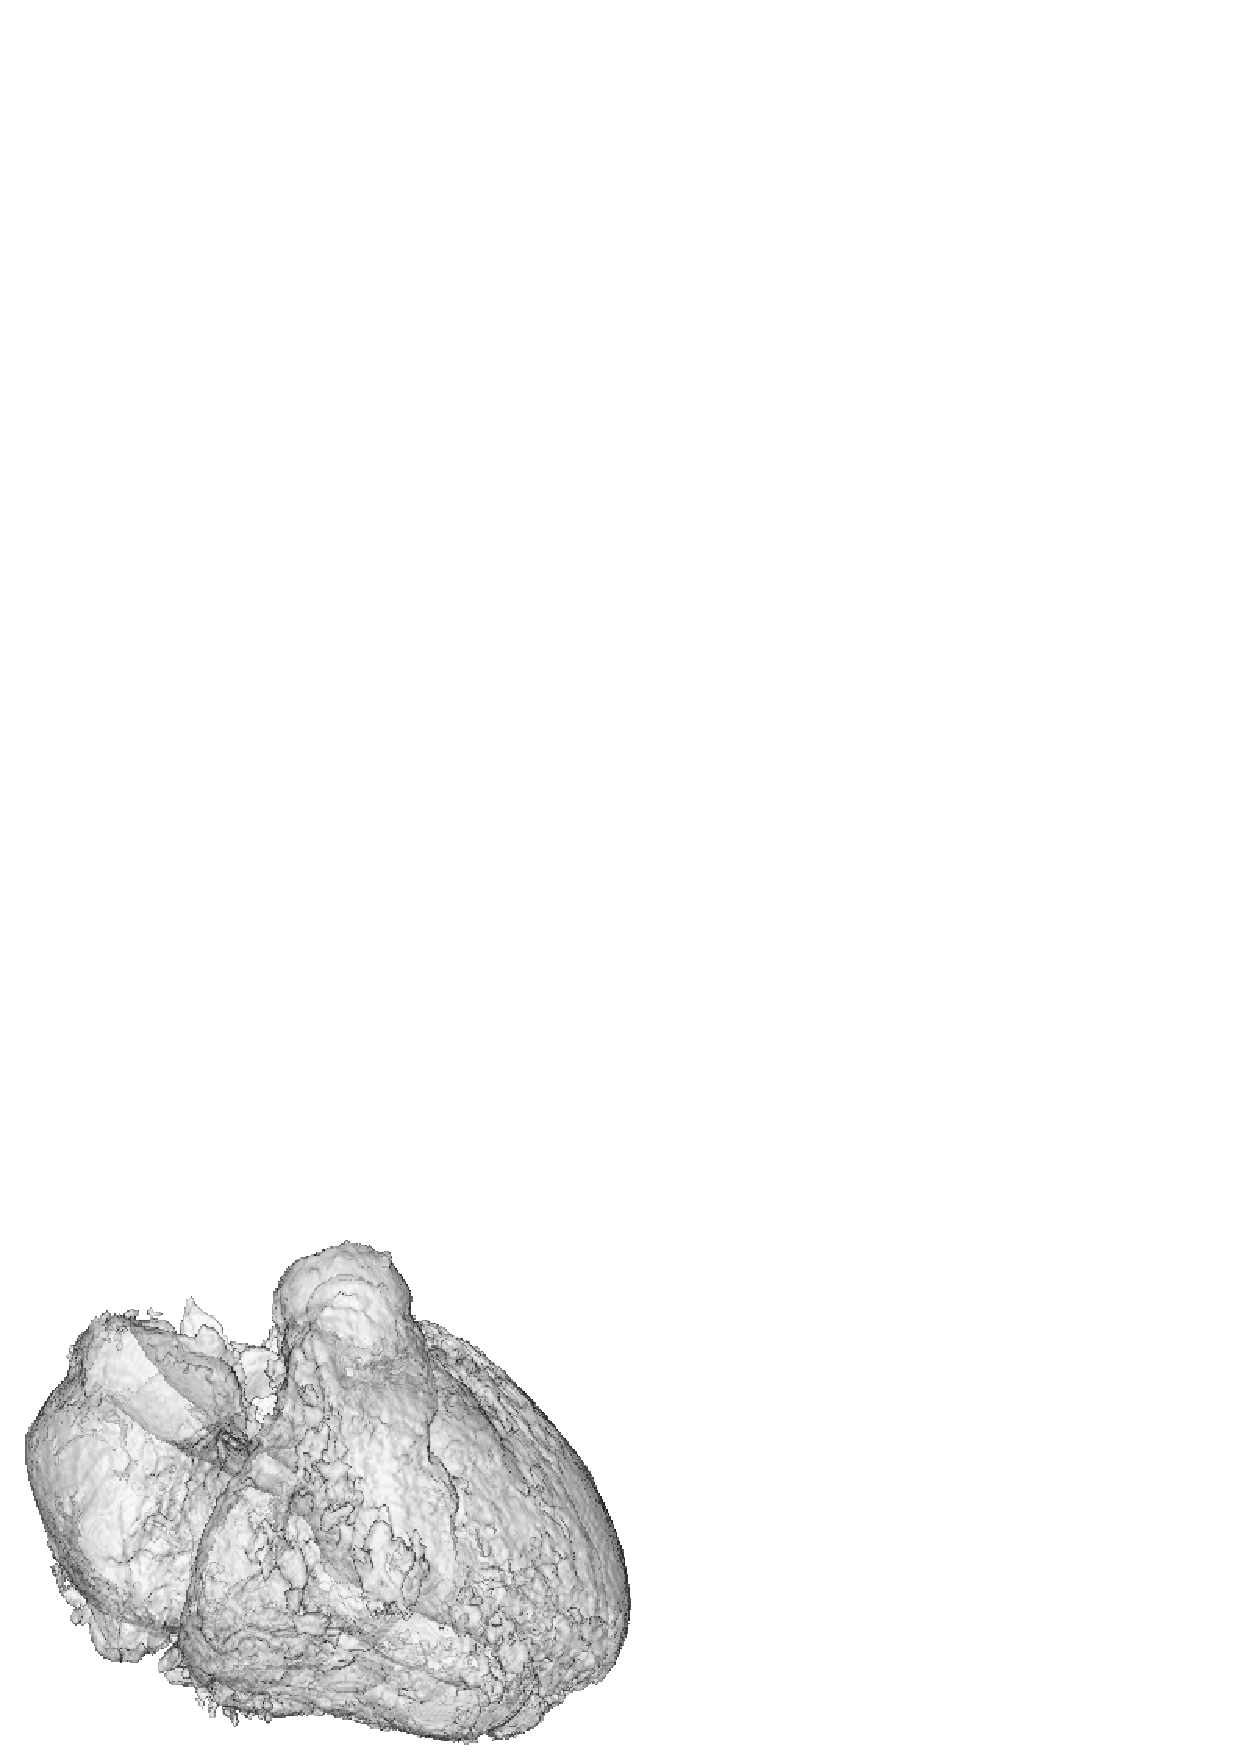
\includegraphics[height=2.4in]{Figures/chap07/heart.pdf}
\caption{The anterior view of the three-dimensional surface model of the heart.}
\label{fig:Heart}
\end{figure}
